\documentclass{article}
\usepackage[utf8]{inputenc}
\usepackage{geometry}
 \geometry{
 a4paper,
 total={170mm,257mm},
 left=20mm,
 top=20mm,
 }
 \usepackage{graphicx}
 \usepackage{titling}
\usepackage{mathptmx}
\usepackage{amsmath, amsthm, amssymb, calrsfs, wasysym, verbatim, bbm, color, graphics}
\usepackage{float}
\usepackage{longtable}
\usepackage{rotating}
\usepackage{adjustbox}
\usepackage{booktabs}
\usepackage{caption}
\usepackage[english]{babel}
\usepackage[table]{xcolor}
\usepackage{multicol}
\usepackage{hyperref}
\usepackage{amsmath}
\usepackage{listings}
\usepackage{pythonhighlight}
\lstnewenvironment{Python}[1][]{\lstset{style=mypython, frame=none, #1}}{}
 

 \title{Data and Information Quality Project
}
\author{Sofia Martellozzo}
\date{January 2023}
 
 \usepackage{fancyhdr}
\fancypagestyle{plain}{%  the preset of fancyhdr 
    \fancyhf{} % clear all header and footer fields
    \fancyfoot[R]{
\includegraphics[width=1.5cm]{logo_polimi.png}}
    \fancyfoot[L]{\thedate}
    \fancyhead[L]{DQ Project}
    \fancyhead[R]{\theauthor}
}
\pagestyle{plain}
\makeatletter
\def\@maketitle{%
  \newpage
  \null
  \vskip 1em%
  \begin{center}%
  \let \footnote \thanks
    {\LARGE \@title \par}%
    \vskip 1em%
    %{\large \@date}%
  \end{center}%
  \par
  \vskip 1em}
\makeatother

\usepackage{lipsum}  
\usepackage{cmbright}

\begin{document}

\maketitle

\noindent\begin{tabular}{@{}ll}
    Student & \theauthor\\
     StudentID &  996215\\
     Student Personal Code & 10623060\\
      & \\
     Project ID & 18\\
     Assigned Dataset & \texttt{letter.csv}\\
     Assigned Task & Classification
\end{tabular}

%----------------------------------------------------%
\section*{Introduction}
The goal of this project is to evaluate how different imputation techniques influence the performance of different classification algorithms on a given dataset.\\\\
The dataset is composed of 2001 samples and 17 labels: 'x-box', 'y-box', 'width', 'high’,  'onpix', 'x-bar', 'y-bar', 'x2bar', 'y2bar', 'xybar', 'x2ybr', 'xy2br', 'x-ege', 'xegvy', 'y-ege', 'yegvx' and 'letter' , that is the target  to predict. The values of the different labels are almost all around 0 and 15, while the target are 26 different letters: 'L', 'F', 'Z', 'T', 'U', 'H', 'Y', 'B', 'R', 'O', 'X', 'S', 'M', 'P', 'K', 'Q', 'V', 'C', ‘W’,  'N', 'G', 'J', 'E', 'A', 'I', 'D' .\\
The dataset is then manipulated in order to obtain various datasets with different amounts of missing (NaN) values. These values are then injected with two different imputation techniques since ML algorithms cannot be executed on incomplete datasets. \\\\The obtained results are then compared in order to evaluate how different imputation techniques influence the ML algorithms' performances.

%---------------------------------------------------%
\section{Setup choices}

\subsection{Chosen ML algorithm}\label{sec:model}
Supervised learning learns a function to make a prediction of a defined label based on the input data. It can be either classifying data into a category (classification problem) or forecasting an outcome (regression algorithms).\\
A classification model identifies which category an object belongs to whereas a regression model predicts a continuous output. Sometimes there is an ambiguous line between classification algorithms and regression algorithms.\\
Many algorithms can be used for both classification and regression, and classification is just a regression model with a threshold applied. When the number is higher than the threshold it is classified as true while lower classified as false. \\\\
Here follows the description of the two ML algorithms selected to solve the classification problem on the {\texttt letter} dataset.
\newpage
\subsubsection*{Support Vector Classifier (SVC)}
\begin{multicols}{2}
\begin{figure}[H]
        \begin{center}
        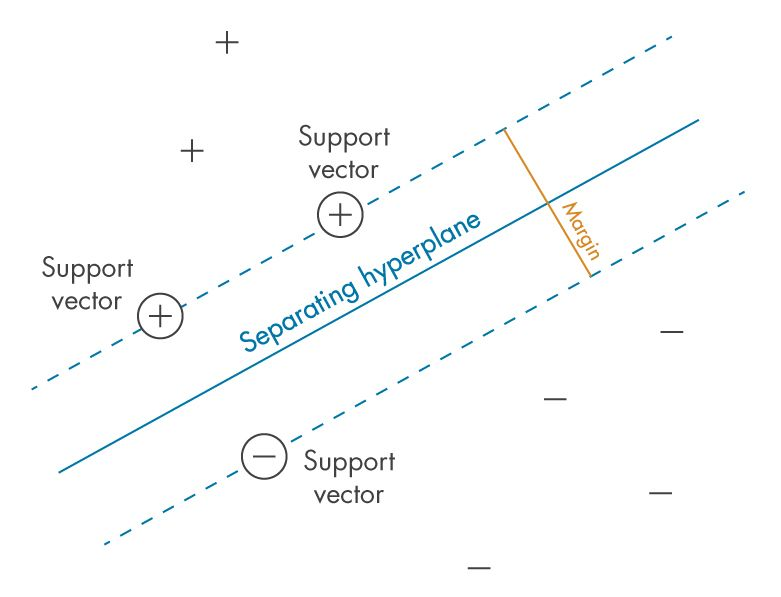
\includegraphics[width=0.4\textwidth]{SVC.jpeg}
        \end{center}
    \end{figure} 
    \columnbreak
\columnbreak
Support Vector Classifier (SVC) is developed based on Support Vector Machine (SVM): a type of deep learning algorithm, builds a learning model that assigns new examples to one group or another. By these functions, SVMs are called a non-probabilistic, binary linear classifier. SVM finds the best way to classify the data based on the position in relation to a border between positive class and negative class. This border is known as the hyperplane which maximize the distance between data points from different classes.
\end{multicols}
\begin{center}
\begin{Python}
# python implementation 
from sklearn.svm import SVC
svc = SVC()
svc.fit(X_train, y_train)
y_pred = svc.predict(X_test)
\end{Python}
\end{center}

\subsubsection*{Decision Tree Classifier}
\begin{multicols}{2}
 \columnbreak
A decision tree is a flowchart-like tree structure where internal nodes represent features (or attributes), branches represent decision rules, and leaf nodes represent outcomes. The tree is partitioned in a recursive manner called recursive partitioning. This flowchart-like structure helps in decision making.\\A decision tree is a white box type of ML algorithm. It shares internal decision-making logic, which is not available in the black box type of algorithms such as Neural Network. Its training time is faster compared to the neural network algorithm.\\ A decision tree builds tree branches in a hierarchy approach and each branch can be considered as an if-else statement. The branches are developed by partitioning the dataset into subsets based on most important features. Final classification happens at the leaves of the decision tree.
\begin{figure}[H]
        \begin{center}
        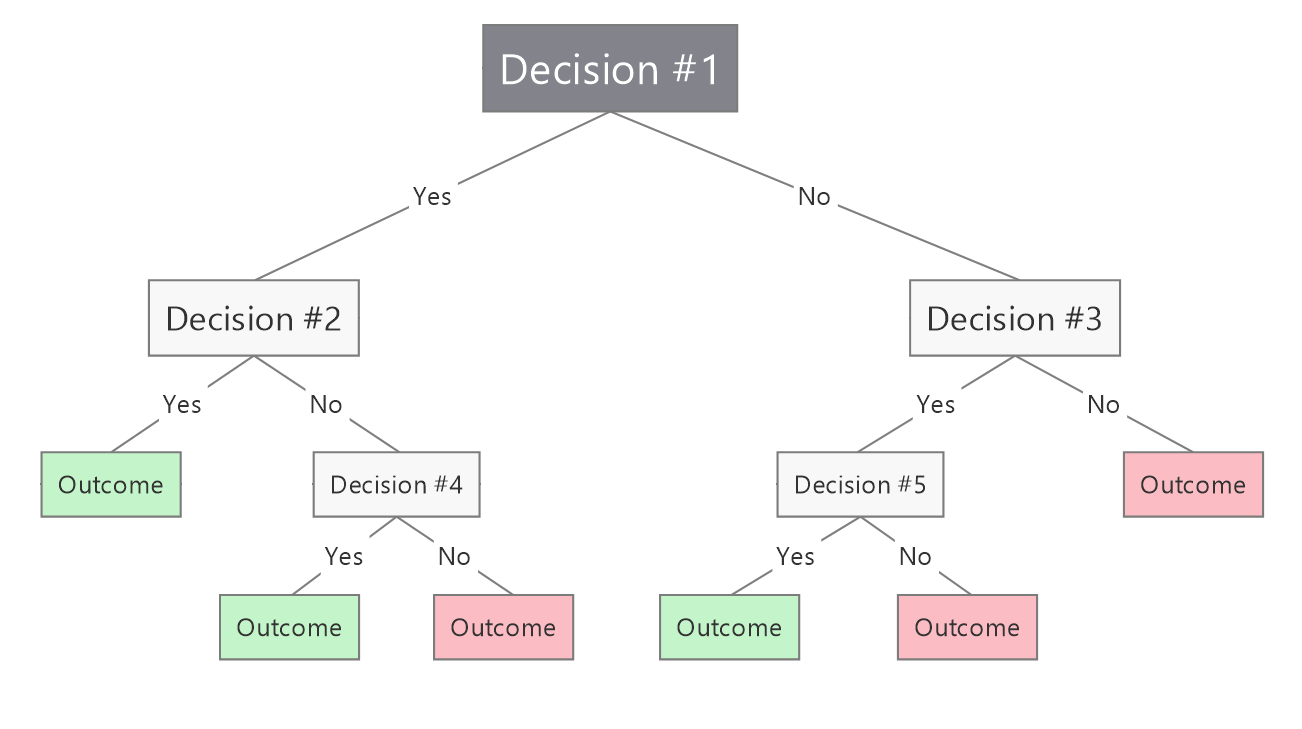
\includegraphics[width=0.5\textwidth]{DecTree.png}
        \end{center}
    \end{figure} 
\end{multicols}
\begin{center}
\begin{Python}
# python implementation 
from sklearn.tree import DecisionTreeClassifier
dtc = DecisionTreeClassifier()
dtc.fit(X_train, y_train)
y_pred = dtc.predict(X_test)
\end{Python}
\end{center}

%----------------------------------------------------%

\subsection{Chosen ML performance evaluation metrics} \label{sec:performances}
In this section is provided a simple description of different metrics used to evaluate the performance of the algorithms implemented for the classification. 

\subsubsection*{Confusion Matrix}
A confusion matrix is used to define the performance of a classification algorithm. It is an especially useful tool in multi-class classification problems. It is a matrix that compares the number of predictions for each class that are correct and those that are incorrect. Each row of the matrix represents the instances in a predicted class, while each column represents the instances in an actual class (or vice versa).\\ The name stems from the fact that it makes it easy to see if the system is confusing two classes (i.e. commonly mislabeling one as another).  
In a confusion matrix, there are 4 values to pay attention to:
\begin{itemize}
    \item True positives: The number of positive observations the model correctly predicted as positive.
    \item False positive: The number of negative observations the model incorrectly predicted as positive.
    \item True negative: The number of negative observations the model correctly predicted as negative.
    \item False negative: The number of positive observations the model incorrectly predicted as negative.
\end{itemize}
The following is an example of confusion matrix taken from this project:
\begin{figure}[H]
        \begin{center}
        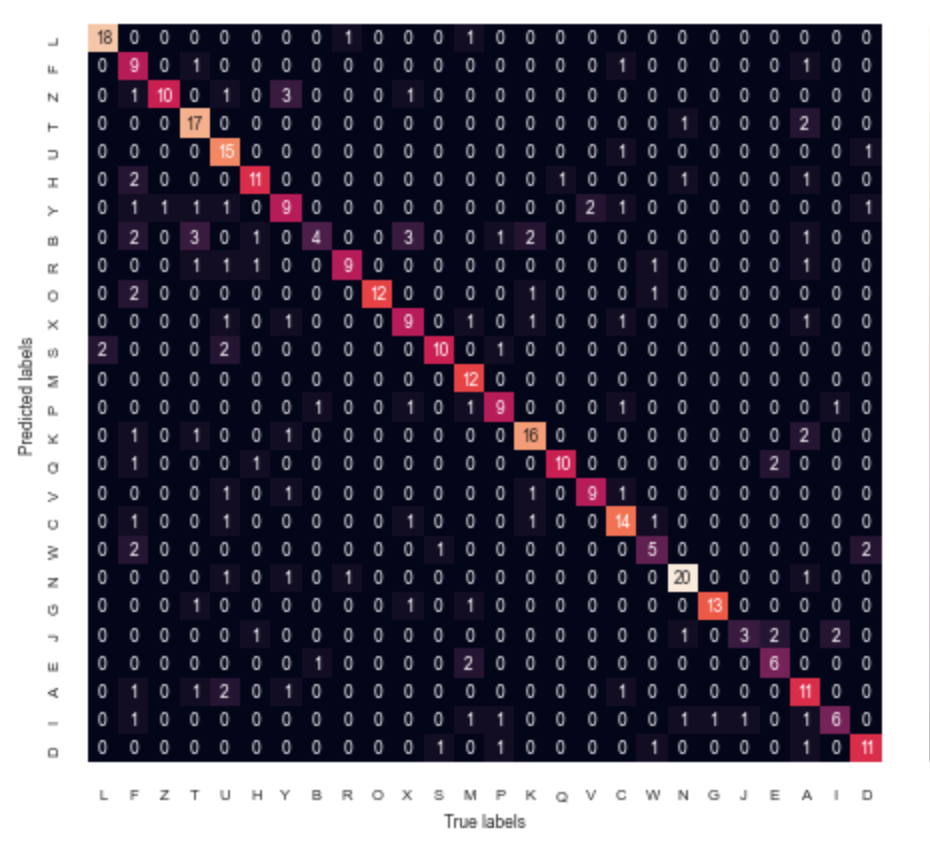
\includegraphics[width=0.33\textwidth]{cm.png}
        \end{center}
\end{figure} 

\subsubsection*{Accuracy}
The overall accuracy of a model is the number of correct predictions divided by the total number of predictions. An accuracy score will give a value between 0 and 1, a value of 1 indicating a perfect model.
\begin{center}
    \begin{math}
Accuracy = \frac{\mbox{Correct Prediction}}{\mbox{Total Predictions}}
\end{math}
\end{center}
It is calculated on all the predicted values (overall accuracy of the model) and also specifically on each label predicted. 

\subsubsection*{Precision}
Precision measures how good the model is at correctly identifying the positive class. In other words out of all predictions for the positive class how many were actually correct?
\begin{center}
    \begin{math}
        Precision = \frac{\mbox{True Positive}}{\mbox{True Positive} + \mbox{False Positive}}
    \end{math}
\end{center}

\subsubsection*{Recall}
Recall measures how good the model is at correctly predicting all the positive observations in the dataset. However, it does not include information about the false positives. 
\begin{center}
    \begin{math}
        Recall = \frac{\mbox{True Positive}}{\mbox{True Positive} + \mbox{False Negative}}
    \end{math}
\end{center}
Usually, precision and recall are observed together. 

\subsubsection*{F1-score}
The F1 score is the harmonic mean of precision and recall. The F1 score will give a number between 0 and 1. If the F1 score is 1.0 this indicates perfect precision and recall. If the F1 score is 0 this means that either the precision or the recall is 0.
\begin{center}
    \begin{math}
        F1-score =\quad \mbox{2} x \quad\dfrac{\mbox{Precision} x \mbox{Recall}}{\mbox{Precision} + \mbox{Recall}} 
    \end{math} 
\end{center}





%---------------------------------------------------%
\subsection{Imputation techniques selected}
Imputation is a technique used to handle missing values in a dataset. It involves replacing missing values with estimated ones, in order to make the data usable for analysis or modeling. There are several imputation techniques that can be used, depending on the nature of the data and the purpose of the analysis.
\subsubsection*{Mode Imputation}
Mode imputation replaces the missing value with the mode of the non-missing values in the same column. It is a simple and straightforward method, but it can introduce bias in the data if the missing values are not missing at random. The steps to perform mode imputation are:
\begin{enumerate}
    \item Identify the missing values in the dataset.
    \item Compute the mode of the feature for the non-missing values.
    \item Replace the missing value with the computed mode.
\end{enumerate}
Mode imputation is a good choice when the data has a large number of observations for the mode. It is important to note that this method will only work when the variable is categorical or ordinal, if the variable is continuous it will not work. 

\subsubsection*{K-Nearest Neighbors (KNN) Imputation}
KNN Imputation is a form of sample imputation that uses the values of similar cases to fill in the missing data. The idea behind KNN imputation is that a point value can be estimated by the average or the mode of the k-nearest points where k is a user-specified parameter. The steps to perform KNN imputation are:
\begin{enumerate}
    \item Identify the missing values in the dataset.
    \item For each missing value, find the k-nearest neighbors based on a distance metric, such as Euclidean distance.
    \item Compute the average or the mode of the feature of the k-nearest neighbors.
    \item Replace the missing value with the computed average or mode.
\end{enumerate}
KNN imputation is a non-parametric method, which means that it does not make any assumptions about the underlying distribution of the data.\\
It is important to note that the choice of k is crucial for the performance of the KNN imputation. If k is too small, the imputed values will be very sensitive to the presence of outliers, if k is too large, the imputed values will be too similar to the overall mean of the variable.\\
Choosing the number of neighbors in a KNN classifier can be done through experimentation. A common approach is to try a range of values for the number of neighbors and evaluate the performance of the classifier using a metric such as accuracy or F1-score. The value for k that results in the best performance is then chosen as the final value for the model.
Since in this case no outliers are present in the dataset, the choice of k ends up in a range of small values, between 3 and 6. With different trials the one that achieves the best results (higher accuracy) is k equal to 3.\\\\
It is important to notice that imputation can introduce bias into the data, so it is important to evaluate the performance of the imputation method and the impact on the analysis or model.

\newpage
%---------------------------------------------------%
\section{Pipeline implementation}
This chapter provides a step by step explanation of how the pipline was implemented.
\begin{enumerate}
    \item After downloading the dataset in the Anaconda environment, explore it to better understand what it contains. As previously stated, it contains 2001 sample of 25 different integer feature and a label, that is a letter.
    \item \begin{multicols}{2}
    An histogram is a graphical representation of the distribution of a dataset that visualizes the frequency of different values in a dataset. In the case of the 'letter' column, a histogram shows the frequency of each letter in the column.\\ Additionally, it is possible to see if the data is balanced or not. A balanced dataset would have similar frequencies for each letter, while an imbalanced dataset would have some letters that appear more frequently than others.\\From the image reported on the right is possible to see that this dataset is slightly unbalanced.
        \columnbreak
        \begin{figure}[H]
            \begin{center}
            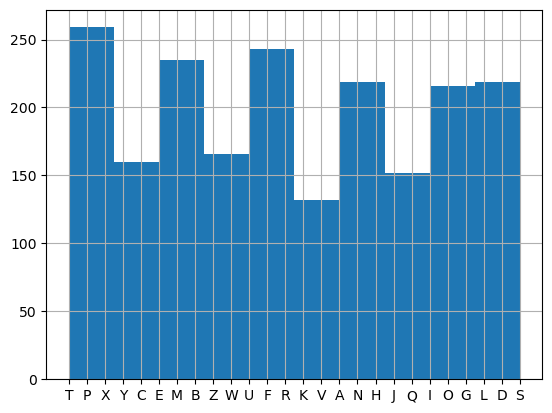
\includegraphics[width=0.34\textwidth]{histogram.png}
            \caption{Histogram of targets}
            \label{fig:hist}
            \end{center}
        \end{figure} 
    \end{multicols}
    \item \begin{multicols}{2}A grouped by chart, also known as a grouped bar chart or a grouped column chart, is a type of chart that is used to compare the values of different categories within a dataset. It is typically used to compare the values of a single variable across different groups or categories.\\ A grouped by chart is similar to a regular bar chart or column chart, but instead of having one bar or column for each data point, it has multiple bars or columns for each data point, grouped together by category.\\Grouped by chart are useful for showing the relationship between multiple variables, especially when the values are being compared across several groups or categories.
    \columnbreak
    \begin{figure}[H]
            \begin{center}
            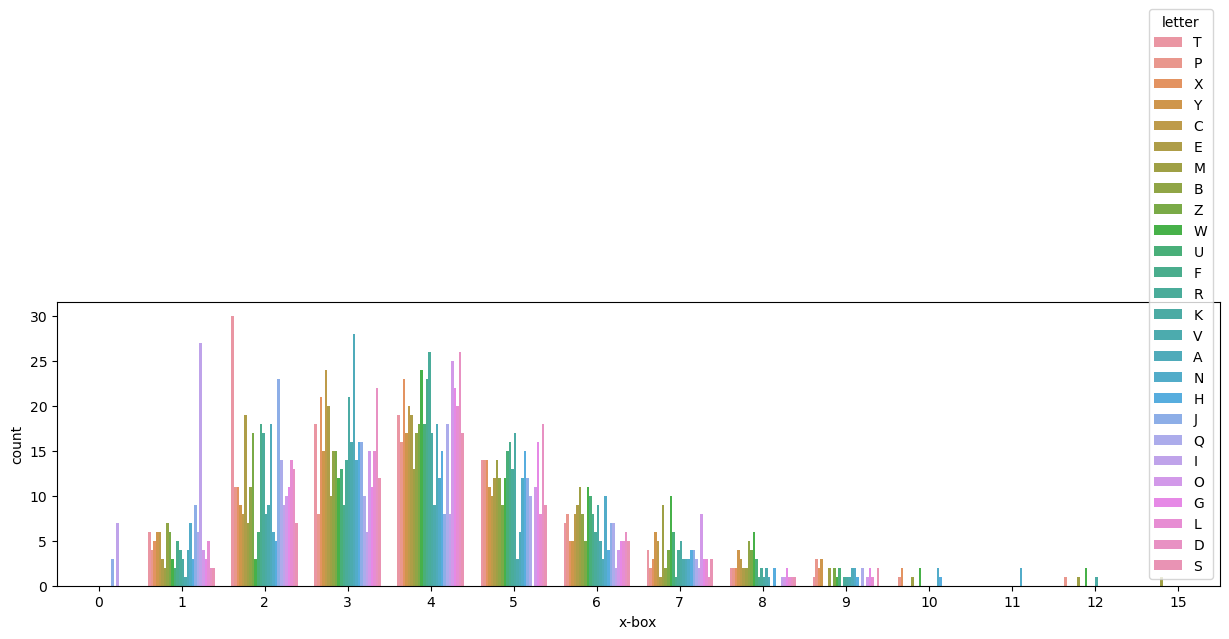
\includegraphics[width=0.4\textwidth]{gbychart.png}
            \caption{Grouped by chart of 'count' feature}
            \end{center}
        \end{figure} 
    \end{multicols}
    \item \begin{multicols}{2}A box plot, also known as a box-and-whisker plot, is a graphical representation of a dataset that shows the distribution of the data. It is a way to visualize the spread and skewness of the data.\\A box plot consists of a box, which represents the interquartile range (IQR) of the data, and whiskers, which extend from the box to show the full range of the data. The box represents the middle 50\% of the data, and the whiskers represent the full range of the data.\\
    In this dataset the values vary significally between the different feature for the different label. 
    \columnbreak
    \begin{figure}[H]
            \begin{center}
            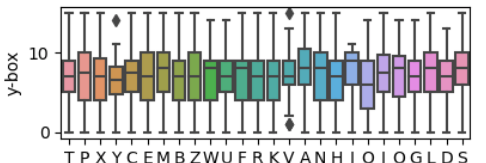
\includegraphics[width=0.4\textwidth]{boxplot.png}
            \caption{Box Plot for 'y-box' feature}
            \label{fig:boxplot}
            \end{center}
        \end{figure}    
    \end{multicols} 
    \item At first, inject randomly in the original dataset provided some NaN values with the provided script.
    \item Save in two lists a copy of the 5 different dirty dataset generated, each list for each imputation technique. Each dataset differentiates from the original one by the percentage of null values: 50\%, 40\%, 30\%, 20\%, 10\% .
    \item Apply both imputation techniques on all the generated datasets, in order to achieve a completeness of 100\%. 
    \item Evaluate the imputation techniques by calculating the accuracy, comparing the generated datasets with the original one. Based on this metric, the k value that gave the best results for the KNN imputation was chosen.
    \item Split all the 10 datasets in Train and Test set, with the function provided by the library \texttt{from sklearn.model\_selection}
    \item Perform the classification on all the datasets with the two implemented algorithms: SVC and Decision Tree Classifier (explained in \ref{sec:model})
    \item Evaluate the performance of the ML algorithm on the results obtained \ref{sec:performances}
\end{enumerate}


%---------------------------------------------------%
\section{Results}
This section provides an overview of the obtained results.
\subsection*{Accuracy on Imputation techniques}
Concerning the Imputation techniques the results obtained are the following:\\
Mode Imputation:
\begin{center}
    \begin{table}[H]
\begin{tabular}{|c|c|c|c|c|c|c|c|c|c|}
\hline
 & x-box & y-box & width & high & onpix & x-bar & y-bar & x2bar & y2bar \\ \hline
dataset1 & 61.7\% & 56.3\% & 61.0\% & 59.8\% & 58.8\% & 64.1\% & 65.5\% & 59.2\% & 58.0\% \\ \hline
dataset2 & 69.1\% & 65.2\% & 67.8\% & 65.0\% & 68.5\% & 72.2\% & 72.4\% & 68.0\% & 67.0\% \\ \hline
dataset3 & 76.7\% & 72.7\% & 77.8\% & 74.0\% & 75.9\% & 80.9\% & 81.4\% & 73.3\% & 77.0\% \\ \hline
dataset4 & 84.4\% & 83.3\% & 84.6\% & 83.6\% & 83.5\% & 85.0\% & 86.1\% & 83.7\% & 83.8\% \\ \hline
dataset5 & 91.8\% & 91.6\% & 92.4\% & 91.8\% & 92.1\% & 93.5\% & 93.2\% & 90.7\% & 91.4\% \\ \hline
\end{tabular}
\end{table}
\begin{table}[H]
\begin{tabular}{|c|c|c|c|c|c|c|c|c|c|}
\hline
 & xybar & x2ybr & xy2br & x-ege & xegvy & y-ege & yegvx & total \\ \hline
dataset1 & 62.8\% & 64.6\% & 67.2\% & 61.3\% & 70.6\% & 59.9\% & 68.5\% & 62.5\% \\ \hline
dataset2 & 71.5\% & 71.6\% & 72.1\% & 69.6\% & 74.8\% & 65.9\% & 76.0\% & 69.8\% \\ \hline
dataset3 & 77.5\% & 79.2\% & 79.5\% & 77.4\% & 82.4\% & 75.5\% & 82.0\% & 77.7\% \\ \hline
dataset4 & 85.4\% & 85.0\% & 86.1\% & 83.6\% & 88.6\% & 84.2\% & 87.7\% & 84.9\% \\ \hline
dataset5 & 92.5\% & 92.8\% & 92.4\% & 91.5\% & 93.7\% & 92.1\% & 93.9\% & 92.3\% \\ \hline
\end{tabular}
\end{table}
\end{center}
The best results are obtained in the first dataset (the one with 50\% of completeness) since, with the imputation are injected 12.5\% of correct values, generating a dataset of 62.5\% of accuracy overall. While the obtained accuracy is satisfying, the improvement on the incomplete dataset is minimal.\\\\
KNN Imputation:
\begin{center}
    \begin{table}[H]
\begin{tabular}{|c|c|c|c|c|c|c|c|c|c|}
\hline
& x-box & y-box & width & high & onpix & x-bar & y-bar & x2bar & y2bar \\ \hline
dataset1 & 54.6\% & 50.6\% & 53.3\% & 53.8\% & 54.1\% & 51.4\% & 55.1\% & 53.0\% & 53.4\% \\ \hline
dataset2 & 64.2\% & 61.6\% & 63.1\% & 61.9\% & 64.9\% & 64.0\% & 65.3\% & 63.8\% & 64.9\% \\ \hline
dataset3 & 73.3\% & 71.1\% & 74.8\% & 72.6\% & 74.7\% & 75.6\% & 77.0\% & 71.3\% & 74.4\% \\ \hline
dataset4 & 82.6\% & 82.7\% & 83.7\% & 82.5\% & 83.7\% & 82.9\% & 84.6\% & 82.9\% & 83.3\% \\ \hline
dataset5 & 91.8\% & 91.3\% & 91.8\% & 91.5\% & 92.6\% & 93.0\% & 92.4\% & 91.7\% & 92.0\% \\ \hline
\end{tabular}
\end{table}
\begin{table}[H]
\begin{tabular}{|c|c|c|c|c|c|c|c|c|c|}
\hline
& xybar & x2ybr & xy2br & x-ege & xegvy & y-ege & yegvx & total \\ \hline
dataset1 & 51.4\% & 52.4\% & 54.7\% & 53.5\% & 58.8\% & 53.5\% & 54.5\% & 53.6\% \\ \hline
dataset2 & 62.5\% & 63.5\% & 63.8\% & 64.0\% & 65.5\% & 62.8\% & 65.3\% & 63.8\% \\ \hline
dataset3 & 74.1\% & 73.6\% & 74.9\% & 75.5\% & 77.7\% & 74.4\% & 77.0\% & 74.5\% \\ \hline
dataset4 & 84.1\% & 83.3\% & 83.9\% & 84.0\% & 86.9\% & 84.8\% & 84.3\% & 83.7\% \\ \hline
dataset5 & 91.6\% & 93.0\% & 92.3\% & 92.7\% & 92.9\% & 92.9\% & 93.2\% & 92.3\% \\ \hline
\end{tabular}
\end{table}
\end{center}
In this case the technique obtains worse performances, imputing just a 3\% of correct data.

\subsection*{Performance of ML algorithms}
The evaluation of the implemented ML algorithms is done through the following performance metrics (explained in \ref{sec:performances}).\\
For all the following performance metrics is reported the results of the prediction on the dataset with Mode imputation followed by the results on the dataset with KNN imputation.
\subsubsection*{Accuracy}
\begin{table}[H]
\begin{tabular}{|c|c|c|c|c|c|}
\hline
 & dataset1 & dataset2 & dataset3 & dataset4 & dataset5 \\ \hline
SVM & 0.319 & 0.377 & 0.499 & 0.596 & 0.693 \\
\hline
Decision Tree & 0.317 & 0.314 & 0.397 & 0.479 & 0.601 \\ \hline
\end{tabular}\\
\begin{tabular}{|c|c|c|c|c|c|}
\hline
 & dataset1 & dataset2 & dataset3 & dataset4 & dataset5 \\ \hline
SVM & 0.319 & 0.377 & 0.499 & 0.596 & 0.693 \\ \hline
Decision Tree & 0.322 & 0.302 & 0.392 & 0.466 & 0.584 \\ \hline
\end{tabular}
\end{table}The results are really similar: both ML algorithms perform quite poorly (30\% of accuracy) in the first dataset. While SVM has the same performances with both imputation techniques, the Decision Tree obtains a slightly worse performance with the KNN imputation.
\subsubsection*{Precision}
\begin{table}[H]
\begin{tabular}{|c|c|c|c|c|c|}
\hline
 & dataset1 & dataset2 & dataset3 & dataset4 & dataset5 \\ \hline
SVM & 0.336 & 0.42 & 0.567 & 0.638 & 0.713 \\ \hline
Decision Tree & 0.305 & 0.31 & 0.403 & 0.481 & 0.592 \\ \hline
\end{tabular}\\
\begin{tabular}{|c|c|c|c|c|c|}
\hline
 & dataset1 & dataset2 & dataset3 & dataset4 & dataset5 \\ \hline
SVM & 0.336 & 0.420 & 0.567 & 0.638 & 0.713 \\ \hline
Decision Tree & 0.321 & 0.298 & 0.391 & 0.465 & 0.579 \\ \hline
\end{tabular}
\end{table}
The same observations can be done for the Precision of the algorithm.
\subsubsection*{Recall}
\begin{table}[H]
\begin{tabular}{|c|c|c|c|c|c|}
\hline
 & dataset1 & dataset2 & dataset3 & dataset4 & dataset5 \\ \hline
SVM & 0.307 & 0.365 & 0.487 & 0.586 & 0.679 \\ \hline
Decision Tree & 0.316 & 0.302 & 0.384 & 0.474 & 0.593 \\ \hline
\end{tabular}\\
\begin{tabular}{|c|c|c|c|c|c|}
\hline
 & dataset1 & dataset2 & dataset3 & dataset4 & dataset5 \\ \hline
SVM & 0.307 & 0.365 & 0.487 & 0.586 & 0.679 \\ \hline
Decision Tree & 0.320 & 0.291 & 0.373 & 0.462 & 0.570 \\ \hline
\end{tabular}
\end{table}
\subsubsection*{F1-score}
\begin{table}[h]
\begin{tabular}{|c|c|c|c|c|c|}
\hline
 & dataset1 & dataset2 & dataset3 & dataset4 & dataset5 \\ \hline
SVM & 0.301 & 0.367 & 0.490 & 0.589 & 0.679 \\ \hline
Decision Tree & 0.303 & 0.300 & 0.386 & 0.471 & 0.588 \\ \hline
\end{tabular}\\
\begin{tabular}{|c|c|c|c|c|c|}
\hline
 & dataset1 & dataset2 & dataset3 & dataset4 & dataset5 \\ \hline
SVM & 0.301 & 0.367 & 0.490 & 0.589 & 0.679 \\ \hline
Decision Tree & 0.311 & 0.289 & 0.375 & 0.456 & 0.569 \\ \hline
\end{tabular}
\end{table}
Even for Recall and F1-score we can say the same as before.
\subsubsection*{Confusion Matrix}
In the notebook is possible to visualize all the confusion matrices generated to evaluate the prediction. From them it is possible to see that not all the labels are wrongly classified: some of them, for example 'L' , have good results. In other cases some labels are even never correctly classified.\\\\
The reason of these results could be in the fact that some classes have a really similar distribution of the values. As we can see by the Box Plot \ref{fig:boxplot} the feature 'y-box' has really similar distribution of the data for almost all the labels. In this situation the classifier could have more difficulties in predicting the class correctly. One possible solution could be normalizing all the data before computing the task with the ML algorithms.\\\\
From the histogram \ref{fig:hist} plotted also for each feature, it is possible to observe that there is not a definite distribution of the data. Many of them look like a Gaussian distribution, but with the mean value 'oversampled', breaking any possible pattern. Another possible solution could be to standardize each feature. Since many features look very similar, another possible solution to improve the performance of the algorithms could be performing a feature selection technique. There are many feature selection techniques, like filter or wrapper,  whose goal is to improve the performance of the model, by reducing the dimensionality of the data and removing irrelevant or redundant features. The choice of the feature selection technique depends on the characteristics of the data and the specific requirements of the problem. It is also common to use an ensemble of different feature selection techniques to find the most informative subset of features.\\
Finally, given the unbalanced nature of the dataset, implementing data augmentation techniques could results in better performances in classifications thanks to a more balanced dataset. 
\end{document}
